% Three Wolfram rules for the review, following the L12b rule-number figure:
% one example of four neighbors for each sum, then the three lookup tables.
% Columns run from c = 8 to c = 0, the order of the base-3 rule digits.
% Every output is decoded from its rule number, not typed independently.
% Checks: R19280 = (222110002)_3; R19286 = (222110022)_3; R0 = (000000000)_3.
% Only c = 1 differs between the first two rules. R0 gives Buy at every sum.
\documentclass[tikz,border=6pt]{standalone}
% Shared style for the L13a schematics (November 12, 2026), \input by each Fig-L13a-*.tex.
% Same fonts, ink, accent colors, boxes, and arrows as the L12a schematics
% (week-12/L12a/figs/abm-diagram.tex), with the plot styles of the L10b profit diagrams
% (arrowed axes, a thick ink curve, open circle markers, dashed drops). The notebook SVG
% carries a dark palette added by theme_svg.py; every color here must be mapped there.
\usepackage[no-math]{fontspec}
\IfFontExistsTF{Arial}{\setsansfont{Arial}}{\setsansfont{TeX Gyre Heros}}
\renewcommand{\familydefault}{\sfdefault}
\usepackage{amsmath,amssymb}
\usetikzlibrary{arrows.meta,calc,positioning,decorations.pathreplacing}

\definecolor{vnink}{HTML}{202124}
\definecolor{gdblue}{HTML}{0091FF}
\definecolor{gdred}{HTML}{E02020}
\definecolor{gdgray}{HTML}{6D7278}
\definecolor{saorange}{HTML}{F08C00}
\definecolor{boxfill}{HTML}{F1F3F4}
\definecolor{orangefill}{HTML}{FFE8C7}
\definecolor{bluefill}{HTML}{E5F3FF}
\definecolor{redfill}{HTML}{FDE8E8}
\definecolor{gridgray}{HTML}{E3E5E8}

\tikzset{
  every picture/.append style={x=1cm, y=1cm, font=\sffamily\small, text=vnink},
  % boxes and arrows, as in the L12a schematics
  flow/.style={draw=vnink, line width=0.9pt, -{Latex[length=2.4mm, width=1.7mm]}},
  feedback/.style={draw=saorange, line width=1.2pt, -{Latex[length=2.6mm, width=1.9mm]}, rounded corners=6pt},
  sumbox/.style={draw=vnink, fill=boxfill, line width=0.8pt, rounded corners=3pt, inner sep=5pt, align=center},
  note/.style={text=gdgray, font=\sffamily\footnotesize, align=center},
  state/.style={circle, draw=vnink, fill=white, line width=1.0pt, minimum size=1.1cm, inner sep=0pt, font=\sffamily\normalsize},
  % plots, as in the L10b profit diagrams
  axis/.style={draw=vnink, line width=0.8pt, -{Latex[length=2.6mm, width=1.8mm]}},
  spine/.style={draw=vnink, line width=0.8pt},
  curve/.style={draw=vnink, line width=1.6pt, line join=round, line cap=round},
  series/.style={draw=gdgray, line width=0.9pt, line join=round},
  drop/.style={draw=gdgray, line width=0.8pt, dash pattern=on 3pt off 2pt},
  pt/.style={circle, draw=vnink, fill=white, line width=1.0pt, inner sep=0pt, minimum size=2.0mm},
}

\definecolor{buyblue}{HTML}{0072B2}
\definecolor{holdgray}{HTML}{AAAAAA}
\definecolor{sellorange}{HTML}{D55E00}
\definecolor{switchfill}{HTML}{FFFDD6}
\newcount\ruledigit
\newcount\rulequotient
\newcount\ruledivisor

\tikzset{
  tile/.style={rectangle,rounded corners=2pt,line width=.8pt,inner sep=0pt,align=center},
  buy/.style={tile,draw=buyblue,fill=buyblue!12},
  hold/.style={tile,draw=holdgray,fill=holdgray!12},
  sell/.style={tile,draw=sellorange,fill=sellorange!15},
  me/.style={tile,draw=vnink,fill=white},
  nb/.style={minimum width=.38cm,minimum height=.38cm,font=\sffamily\scriptsize},
  output/.style={minimum width=.92cm,minimum height=.69cm,font=\sffamily\small},
  lookup/.style={draw=gdgray,line width=.7pt,-{Latex[length=1.7mm,width=1.2mm]}},
}

\begin{document}
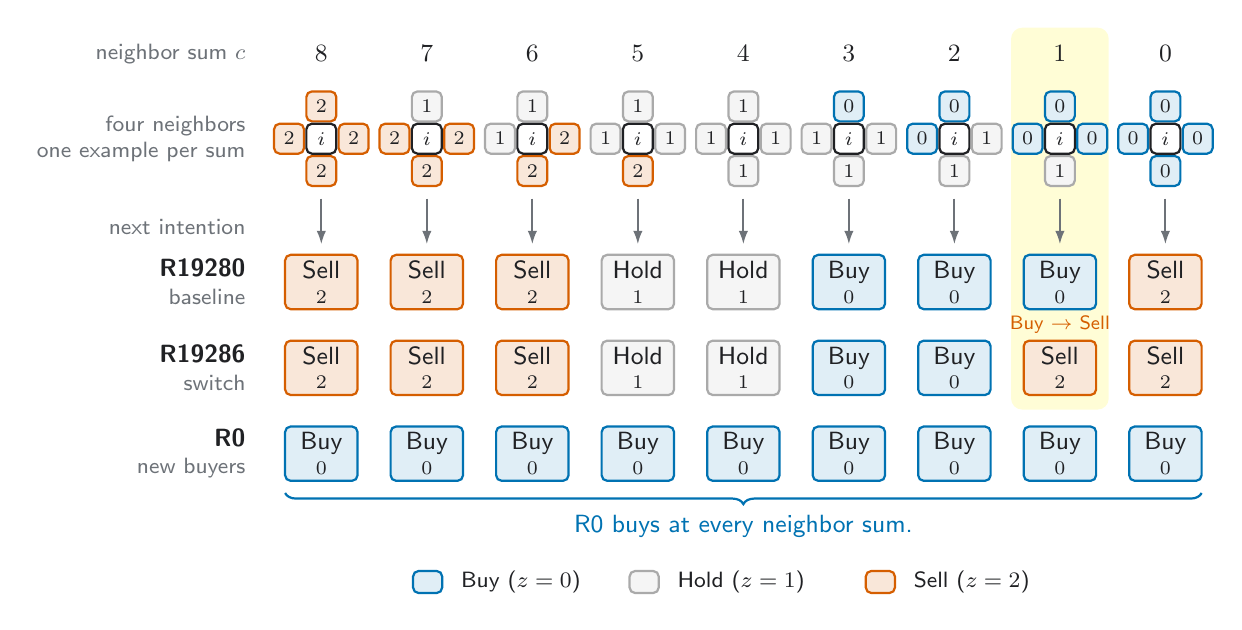
\begin{tikzpicture}
\def\pitch{1.34}
\def\ns{.41}
\def\ysum{5.85}
\def\ynb{4.77}
\def\ya{2.95}
\def\yb{1.86}
\def\yc{.77}
\pgfmathsetmacro{\hx}{7*\pitch}

% One quiet band links the worked neighbor pattern to the only changed entry.
\fill[switchfill,rounded corners=4pt] (\hx-.62,1.33) rectangle (\hx+.62,6.18);
\node[anchor=east,font=\sffamily\footnotesize,text=gdgray] at (-.84,\ysum) {neighbor sum $c$};
\node[anchor=east,align=right,font=\sffamily\footnotesize,text=gdgray] at (-.84,\ynb)
  {four neighbors\\one example per sum};
\node[anchor=east,align=right,font=\sffamily\footnotesize,text=gdgray] at (-.84,3.65)
  {next intention};

% The same neighbor crosses as the L12b lecture, with the trader in the center.
\foreach \col/\c/\north/\west/\east/\south in {
  0/8/2/2/2/2,
  1/7/1/2/2/2,
  2/6/1/1/2/2,
  3/5/1/1/1/2,
  4/4/1/1/1/1,
  5/3/0/1/1/1,
  6/2/0/0/1/1,
  7/1/0/0/0/1,
  8/0/0/0/0/0} {
  \pgfmathsetmacro{\xc}{\col*\pitch}
  \node[font=\sffamily\bfseries\small] at (\xc,\ysum) {$\c$};
  \foreach \dg/\dx/\dy in {\north/0/1,\west/-1/0,\east/1/0,\south/0/-1} {
    \ifcase\dg\def\st{buy}\or\def\st{hold}\or\def\st{sell}\fi
    \node[\st,nb] at (\xc+\dx*\ns,\ynb+\dy*\ns) {$\dg$};
  }
  \node[me,nb] at (\xc,\ynb) {$i$};
  \draw[lookup] (\xc,\ynb-.76) -- (\xc,\ya+.48);

  % Decode each rule at this sum using exact integer division.
  \foreach \ruleindex/\yy in {19280/\ya,19286/\yb,0/\yc} {
    \pgfmathtruncatemacro{\power}{pow(3,\c)}
    \ruledivisor=\power\relax
    \ruledigit=\ruleindex\relax
    \divide\ruledigit by \ruledivisor
    \rulequotient=\ruledigit
    \divide\rulequotient by 3
    \multiply\rulequotient by 3
    \advance\ruledigit by -\rulequotient
    \edef\state{\the\ruledigit}
    \ifcase\state\def\style{buy}\def\word{Buy}\or
      \def\style{hold}\def\word{Hold}\or
      \def\style{sell}\def\word{Sell}\fi
    \node[\style,output] at (\xc,\yy) {\word\\[-2pt]{\scriptsize $\state$}};
  }
}

% Rule names and roles share the same baseline and left edge.
\foreach \yy/\ruleindex/\role in {\ya/19280/baseline,\yb/19286/switch,\yc/0/new buyers} {
  \node[anchor=east,align=right] at (-.84,\yy)
    {\textbf{R\ruleindex}\\[-1pt]{\footnotesize\color{gdgray}\role}};
}

% The highlighted entry explains the switch; the third row explains R0 directly.
\node[align=center,font=\sffamily\scriptsize,text=sellorange]
  at (\hx,2.405) {Buy $\to$ Sell};
\draw[draw=buyblue,line width=.8pt,decorate,decoration={brace,mirror,amplitude=4pt}]
  (-.46,.27) -- (8*\pitch+.46,.27);
\node[font=\sffamily\small,text=buyblue] at (4*\pitch,-.15)
  {R0 buys at every neighbor sum.};

% A compact key keeps the numeric intention codes explicit.
\foreach \xx/\st/\label in {1.35/buy/Buy ($z=0$),4.1/hold/Hold ($z=1$),7.1/sell/Sell ($z=2$)} {
  \node[\st,minimum width=.37cm,minimum height=.28cm] at (\xx,-.86) {};
  \node[anchor=west,font=\sffamily\footnotesize] at (\xx+.3,-.86) {\label};
}
\end{tikzpicture}
\end{document}
